% !TeX encoding = UTF-8
% !TeX program = xelatex
% !TeX spellcheck = en_US

\documentclass[degree=doctor]{thuthesis}
  % 学位 degree:
  %   doctor | master | bachelor | postdoc
  % 学位类型 degree-type:
  %   academic(默认)| professional
  % 语言 language
  %   chinese(默认)| english
  % 字体库 fontset
  %   windows | mac | fandol | ubuntu
  % 建议终版使用 Windows 平台的字体编译

% 论文基本配置,加载宏包等全局配置
% !TeX root = ./thuthesis-example.tex

% 论文基本信息配置

\thusetup{
  %******************************
  % 注意:
  %   1. 配置里面不要出现空行
  %   2. 不需要的配置信息可以删除
  %   3. 建议先阅读文档中所有关于选项的说明
  %******************************
  %
  % 输出格式
  %   选择打印版(print)或用于提交的电子版(electronic),前者会插入空白页以便直接双面打印
  %
  output = print,
  %
  % 标题
  %   可使用“\\”命令手动控制换行
  %
  title  = {这是中文标题},
  title* = {The English title},
  %
  % 学科门类
  %   1. 学术型
  %      - 中文
  %        需注明所属的学科门类,例如:
  %        哲学、经济学、法学、教育学、文学、历史学、理学、工学、农学、医学、
  %        军事学、管理学、艺术学
  %      - 英文
  %        博士:Doctor of Philosophy
  %        硕士:
  %          哲学、文学、历史学、法学、教育学、艺术学门类,公共管理学科
  %          填写“Master of Arts“,其它填写“Master of Science”
  %   2. 专业型
  %      直接填写专业学位的名称,例如:
  %      教育博士、工程硕士等
  %      Doctor of Education, Master of Engineering
  %   3. 本科生不需要填写
  %
  degree-category  = {医学博士},
  degree-category* = {Medical Doctor},
  %
  % 培养单位
  %   填写所属院系的全名
  %
  department = {清华大学医学院},
  %
  % 学科
  %   1. 研究生学术型学位,获得一级学科授权的学科填写一级学科名称,其他填写二级学科名称
  %   2. 本科生填写专业名称,第二学位论文需标注“(第二学位)”
  %
  discipline  = {临床医学专业2015级},
  discipline* = {Tsinghua M.D. Program},
  %
  % 专业领域
  %   1. 设置专业领域的专业学位类别,填写相应专业领域名称
  %   2. 2019 级及之前工程硕士学位论文,在 `engineering-field` 填写相应工程领域名称
  %   3. 其他专业学位类别的学位论文无需此信息
  %
  % professional-field  = {计算机技术},
  % professional-field* = {Computer Technology},
  %
  % 姓名
  %
  author  = {王小五},
  author* = {Xiaowu Wang},
  %
  % 指导教师
  %   中文姓名和职称之间以英文逗号“,”分开,下同
  %
  supervisor  = {某, 教授},
  supervisor* = {Professor X, yz},
  %
  % 副指导教师
  %
  associate-supervisor  = {某, 教授},
  associate-supervisor* = {Professor Y, xz},
  %
  % 联合指导教师
  %
  % co-supervisor  = {某某某, 教授},
  % co-supervisor* = {Professor Mou Moumou},
  %
  % 日期
  %   使用 ISO 格式;默认为当前时间
  %
  date = {2023-11-12},
  %
  % 是否在中文封面后的空白页生成书脊(默认 false)
  %
  include-spine = true,
  spine-font = {\zihao{3}},
  spine-title = {基于xxx},
  spine-author = {王小五},
  %
  % 密级和年限
  %   秘密, 机密, 绝密
  %
  % secret-level = {秘密},
  % secret-year  = {10},
  %
  % 博士后专有部分
  %
  % clc                = {分类号},
  % udc                = {UDC},
  % id                 = {编号},
  % discipline-level-1 = {计算机科学与技术},  % 流动站(一级学科)名称
  % discipline-level-2 = {系统结构},          % 专业(二级学科)名称
  % start-date         = {2011-07-01},        % 研究工作起始时间
}

% 载入所需的宏包 
\usepackage[sectionbib]{bibunits}
\usepackage{titlesec}
% 定理类环境宏包
\usepackage{amsthm}

% 也可以使用 ntheorem
% \usepackage[amsmath,thmmarks,hyperref]{ntheorem}

\thusetup{
  %
  % 数学字体
  % math-style = GB,  % GB | ISO | TeX
  math-font  = xits,  % stix | xits | libertinus
}
\thusetup{language=english}
% 可以使用 nomencl 生成符号和缩略语说明
% \usepackage{nomencl}
% \makenomenclature

% 表格加脚注
\usepackage{threeparttable}

% 表格中支持跨行
\usepackage{multirow}

% 固定宽度的表格。
% \usepackage{tabularx}

% 跨页表格
\usepackage{longtable}

% 算法
\usepackage{algorithm}
\usepackage{algorithmic}

% 量和单位
\usepackage{siunitx}

% 参考文献使用 BibTeX + natbib 宏包
% 顺序编码制
% \usepackage[sort]{natbib}
% \bibliographystyle{thuthesis-numeric}

% 著者-出版年制
% \usepackage{natbib}
% \bibliographystyle{thuthesis-author-year}

% 本科生参考文献的著录格式
% \usepackage[sort]{natbib}
% \bibliographystyle{thuthesis-bachelor}

% Cell Journals
\usepackage[sort]{natbib}
\bibliographystyle{cell}

% 参考文献使用 BibLaTeX 宏包
% \usepackage[style=thuthesis-numeric]{biblatex}
% \usepackage[style=thuthesis-author-year]{biblatex}
% \usepackage[style=gb7714-2015]{biblatex}
% \usepackage[style=apa]{biblatex}
% \usepackage[style=mla-new]{biblatex}
% 声明 BibLaTeX 的数据库
% \addbibresource{ref/refs.bib}

% 定义所有的图片文件在 figures 子目录下
\graphicspath{{figures/}}

% 数学命令
\makeatletter
\newcommand\dif{%  % 微分符号
  \mathop{}\!%
  \ifthu@math@style@TeX
    d%
  \else
    \mathrm{d}%
  \fi
}
\makeatother

% hyperref 宏包在最后调用
\usepackage{hyperref}




\begin{document}

% 封面
\maketitle

% 学位论文指导小组、公开评阅人和答辩委员会名单
% 本科生不需要
% !TeX root = ../thuthesis-example.tex

\begin{committee}[name={毕业论文公开评阅人和答辩委员会名单}]

  \newcolumntype{C}[1]{@{}>{\centering\arraybackslash}p{#1}}

  \section*{公开评阅人名单}

  \begin{center}
    \begin{tabular}{C{3cm}C{3cm}C{9cm}@{}}
      刘XX & 教授   & 清华大学                    \\
      陈XX & 副教授 & XXXX大学                    \\
      杨XX & 研究员 & 中国XXXX科学院XXXXXXX研究所 \\
    \end{tabular}
  \end{center}


  \section*{答辩委员会名单}

  \begin{center}
    \begin{tabular}{C{2.75cm}C{2.98cm}C{4.63cm}C{4.63cm}@{}}
      主席 & 赵XX                  & 教授                    & 清华大学       \\
      委员 & 刘XX                  & 教授                    & 清华大学       \\
          & \multirow{2}{*}{杨XX} & \multirow{2}{*}{研究员} & 中国XXXX科学院 \\
          &                       &                         & XXXXXXX研究所  \\
          & 黄XX                  & 教授                    & XXXX大学       \\
          & 周XX                  & 副教授                  & XXXX大学       \\
      秘书 & 吴XX                  & 助理研究员              & 清华大学       \\
    \end{tabular}
  \end{center}

\end{committee}



% 也可以导入 Word 版转的 PDF 文件
% \begin{committee}[file=figures/committee.pdf]
% \end{committee}


% 使用授权的说明
\copyrightpage
% 将签字扫描后授权文件 scan-copyright.pdf 替换原始页面
% \copyrightpage[file=scan-copyright.pdf]

\frontmatter
% !TeX root = ../thuthesis-example.tex

% 中英文摘要和关键字
\renewcommand{\chaptermark}[1]{\markboth{#1}{}} 
\begin{abstract}
  \markboth{摘要}{}
  肿瘤异质性
  % 关键词用“英文逗号”分隔,输出时会自动处理为正确的分隔符
  \thusetup{
    keywords = {异质性, 精准医疗},
  }
\end{abstract}

\renewcommand{\chaptermark}[1]{\markboth{#1}{}} 
\begin{abstract*}
  \markboth{Abstract}{}
  Tumor heterogeneity
  This paper aims for 
  % Use comma as separator when inputting
  \thusetup{
    keywords* = {heterogeneity, precision medicine},
  }
\end{abstract*}


% 目录
\tableofcontents

% 插图和附表清单
% 本科生的插图索引和表格索引需要移至正文之后、参考文献前
% \listoffiguresandtables  % 插图和附表清单(仅限研究生)
\listoffigures           % 插图清单
\listoftables            % 附表清单

% 符号对照表
% !TeX root = ../thuthesis-example.tex

\begin{denotation}[3cm]
  \item[BC]	breast cancer 
  \item[LN]	lymph node
  \item[SUM44]	SUM44-PE cell line
  \item[MM134]	MDA-MB-134 cell line
  \item[GEMM]	genetically engineered mouse model
  \item[FFPE]	formalin-fixed and paraffin-embedded
  \item[TME]	tumor microenvironment
  \item[PAM50]	Prosigna Molecular 50
  \item[ITH]	intra-tumor heterogeneity
  \item[NGS]	next-generation sequencing
  \item[WGS]	whole genome sequencing
  \item[WES]	whole exome sequencing
  \item[Indel]	short insertion and deletion in genome
  \item[CNA]	copy number alteration
  \item[LOH]	loss of heterozygosity
  \item[3C]	chromosome conformation capture
  \item[ChIP-seq]	chromatin immunoprecipitation sequencing
  \item[WGBS]	whole-genome bisulfite sequencing
  \item[ATAC-seq]	Assay for Transposase-Accessible Chromatin using sequencing
  \item[RNA-seq]	RNA-sequencing
  \item[scRNA-seq]	single cell RNA sequencing
  \item[CyTOF]	mass cytometry
  \item[FACS]	fluorescence-activated cell sorting 
  \item[PCA]	principle component analysis
  \item[t-SNE]	t-Distributed Stochastic Neighbor Embedding
  \item[UMAP]	Uniform Manifold Approximation and Projection
  \item[CRISPR]	clustered regularly interspersed short palindromic repeat
  \item[CAS9]	CRISPR-associated protein 9
  \item[IHC]	immunohistochemistry
  \item[RT-PCR]	reverse transcription polymerase chain reaction
  \item[qPCR]	quantitative polymerase chain reaction
  \item[WB]	western blot
  \item[Dual-Luc]	dual-luciferase reporter assay
  \item[CTD2]	Cancer Target Discovery and Development
\end{denotation}



% 也可以使用 nomencl 宏包,需要在导言区
% \usepackage{nomencl}
% \makenomenclature

% 在这里输出符号说明
% \printnomenclature[3cm]

% 在正文中的任意为都可以标题
% \nomenclature{PI}{聚酰亚胺}
% \nomenclature{MPI}{聚酰亚胺模型化合物,N-苯基邻苯酰亚胺}
% \nomenclature{PBI}{聚苯并咪唑}
% \nomenclature{MPBI}{聚苯并咪唑模型化合物,N-苯基苯并咪唑}
% \nomenclature{PY}{聚吡咙}
% \nomenclature{PMDA-BDA}{均苯四酸二酐与联苯四胺合成的聚吡咙薄膜}
% \nomenclature{MPY}{聚吡咙模型化合物}
% \nomenclature{As-PPT}{聚苯基不对称三嗪}
% \nomenclature{MAsPPT}{聚苯基不对称三嗪单模型化合物,3,5,6-三苯基-1,2,4-三嗪}
% \nomenclature{DMAsPPT}{聚苯基不对称三嗪双模型化合物(水解实验模型化合物)}
% \nomenclature{S-PPT}{聚苯基对称三嗪}
% \nomenclature{MSPPT}{聚苯基对称三嗪模型化合物,2,4,6-三苯基-1,3,5-三嗪}
% \nomenclature{PPQ}{聚苯基喹噁啉}
% \nomenclature{MPPQ}{聚苯基喹噁啉模型化合物,3,4-二苯基苯并二嗪}
% \nomenclature{HMPI}{聚酰亚胺模型化合物的质子化产物}
% \nomenclature{HMPY}{聚吡咙模型化合物的质子化产物}
% \nomenclature{HMPBI}{聚苯并咪唑模型化合物的质子化产物}
% \nomenclature{HMAsPPT}{聚苯基不对称三嗪模型化合物的质子化产物}
% \nomenclature{HMSPPT}{聚苯基对称三嗪模型化合物的质子化产物}
% \nomenclature{HMPPQ}{聚苯基喹噁啉模型化合物的质子化产物}
% \nomenclature{PDT}{热分解温度}
% \nomenclature{HPLC}{高效液相色谱(High Performance Liquid Chromatography)}
% \nomenclature{HPCE}{高效毛细管电泳色谱(High Performance Capillary lectrophoresis)}
% \nomenclature{LC-MS}{液相色谱-质谱联用(Liquid chromatography-Mass Spectrum)}
% \nomenclature{TIC}{总离子浓度(Total Ion Content)}
% \nomenclature{\textit{ab initio}}{基于第一原理的量子化学计算方法,常称从头算法}
% \nomenclature{DFT}{密度泛函理论(Density Functional Theory)}
% \nomenclature{$E_a$}{化学反应的活化能(Activation Energy)}
% \nomenclature{ZPE}{零点振动能(Zero Vibration Energy)}
% \nomenclature{PES}{势能面(Potential Energy Surface)}
% \nomenclature{TS}{过渡态(Transition State)}
% \nomenclature{TST}{过渡态理论(Transition State Theory)}
% \nomenclature{$\increment G^\neq$}{活化自由能(Activation Free Energy)}
% \nomenclature{$\kappa$}{传输系数(Transmission Coefficient)}
% \nomenclature{IRC}{内禀反应坐标(Intrinsic Reaction Coordinates)}
% \nomenclature{$\nu_i$}{虚频(Imaginary Frequency)}
% \nomenclature{ONIOM}{分层算法(Our own N-layered Integrated molecular Orbital and molecular Mechanics)}
% \nomenclature{SCF}{自洽场(Self-Consistent Field)}
% \nomenclature{SCRF}{自洽反应场(Self-Consistent Reaction Field)}



% 正文部分
\mainmatter
\% !TeX root = ../thuthesis-example.tex
\thusetup{
  cite-style = author-year,
}
\noindent
\chapter{Introduction}

\section{Motivation}

Cancer is the leading cause of lethality worldwide, as a byproduct of modern-world longevity – it arises from naturally accumulating mutations, which eventually lead to uncontrollable growth of malignant cells. Cancer is generally classified by tissues of origin, but past decades of molecular biology development have enabled recognition of finer subtypes - each with distinct phenotypes, prognosis, and thus specific treatment. Tumor heterogeneity (TH) emphasizes such variations - as differences between (inter) or within (intra) tumors. It develops via two factors – genomic / epigenetic aberrations (intrinsic), and microenvironment signals (extrinsic) - mutants appear intrinsically and evolve under selective pressure, while successfully expanded clones recruit vessels or suppress immune activities, and thus in turn modify the environment. Given such dynamic heterogeneity, this resultant repertoire may well preserve clones with high invasiveness  to cause metastasis, or high adaptation to cause resistance -altogether posing great challenges to cancer treatment.

Genomic or epigenomics factors are the most recognized contributors to TH. Genetic aberrations result mostly from genomic instability – aberrant ploidy, structural variants, indels or point mutations, arising from mitosis errors or DNA repair deficiency. Among numerous mutations, the specific group of ‘drivers’ are of particular interest, as they greatly promote cancer growth, proliferation or invasiveness – e.g., by hyper-activation of oncogenes (e.g., PI3Ks, MYC, CDKs) and loss of function of tumor suppressor genes (TSG) (e.g., TP53, RB1). Epigenetic states are influenced by both genetic mutations (e.g., chromatin modifiers, transcriptional factors or co-factors) or environment – and are shown as hyper/hypo histone methylation/acetylation, altered 3D chromosome structure, and different chromatin accessibility. These may cause aberrant gene expression - e.g. TSG (CDKN2A, APC, MLH1) silencing by increased promoter CpG and H3K9 methylation, and oncogene (c-Myc, MAGE, CDH3) activation by decreased methylation at promoter CpG islands \citep{cheung2009dna}. Besides these two factors which are relatively stable, cells also render great plasticity, in case of stimulations in particular. These responses are also largely heterogeneous – as reflected by transcriptomic or proteomics profiles, and can equally influence cancer adaptation and evolution as genetic/epigenetic factors.

Multiple techniques are available in measuring tumor heterogeneity – the most well-known example being large cohort studies like TCGA, which used microarrays or bulk RNA sequencing to identify molecular subtypes; as well as the large scale DNA sequencing by ICGC (International Cancer Genome Consortium) or PCAWG (Pan-Cancer Analysis of Whole Genome). Moreover, epigenetics can also be profiled - ChIP-seq identifies sequence bound to histone markers (H3K27ac, H3K27me3, H3K4me1, H3K4me3, H3K9me3) or other transcriptional factors of interest; methylation states can be detected with bisulfate sequencing (WGBS (whole-genome bisulfate sequencing), RRBS (reduced-representation bisulfite sequencing)) or microarray (Illumina Infinium BeadChip); while DNAase-I-seq or ATAC-seq can be used to assess chromatin accessibility. Expression and of total and phosphorylated proteins can be quantified as well – e.g., by RPPA (reverse phase protein array) by using hundreds of antibodies. However, these measurements only resolve phenotypes at tumor level as a mixture of all tumor and/or TME components, in which case intra-tumor heterogeneity (ITH) is not directly explored, and might influence bulk sequencing due to purity issues. To solve this problem, multiple computational methods have been developed, e.g., to dissect clonal states from the bulk DNA-seq data \citep{roth2014pyclone}, SubcloneSeeker \citep{qiao2014subcloneseeker}, or to deconvolute bulk RNA-seq (CIBERSORT \citep{chen2018profiling}, ESTIMATE \citep{yoshihara2013inferring}). But they are nevertheless limited by performance uncertainty which may be data specific. On the other hand, single cell sequencing has developed rapidly during the past decade, for either single omic (scDNA-seq, scATAC-seq, scRNA-seq, CyTOF \citep{bendall2011single}), or multi-omics within the same cell (DR-seq \citep{dey2015integrated}, G\&T-seq \citep{macaulay2015g}, scTrio-seq \citep{hou2016single}, scMT-seq \citep{hu2016simultaneous}) – these techniques thus greatly promote ITH research. 

The ultimate goal of heterogeneity characterization is to suggest personalized therapies targeting pathogenic subclones with driver mutations or transcriptomic signatures, which could then be tested in in vitro (organoids) or in vivo (xenografts) preclinical models. These features can also be traced longitudinally by liquid biopsy, to monitor recurrence, assess responsiveness and guide further decisions.

In summary, tumor heterogeneity extensively exists and greatly contributes to cancer resistance and mortality. Bulk or single cell sequencing can be used for studying inter and intra TH, to identify pathognomonic mechanisms and suggest personalized therapies. Towards this direction, great efforts and achievements have been made, especially in breast cancer - these will be elaborated in the later sections.

\section{Background and Significance}

Breast cancer (BC) is the most common cancer in women worldwide, and the second leading cause of cancer mortality in women in the United States (US). In 2019, there were over 270,000 new diagnosis and more than 42,000 deaths in US. BC is therefore an essential public health issue calling for better prevention, diagnosis and treatment strategies.

During the past decades, research and treatment of BC have both greatly developed, with survival tremendously improved. Current management of primary BC starts with TNM staging and subtyping at diagnosis. Subtyping usually include histopathology and marker expression (ER (estrogen receptor), PR (progesterone receptor), HER2 (human epidermal growth factor receptor 2)) by IHC (immunohistochemistry). Molecular diagnostic by microarray is also applicable to evaluate risk of recurrence (e.g., MammaPrint \citep{cardoso201670}. Regarding treatment, surgery removal is still a primary option, followed by adjuvant therapeutics of endocrine, chemo, targeting, or immune therapies, based on diagnostic features accordingly.

Most (70\%) early-staged primary BC never relapse after surgery and adjuvant therapy. However, for those 30\% who do relapse, distant dissemination composed of multiple subclones usually occurs, followed by the rapid development of resistance and eventually mortality, thus making therapeutics particularly difficult. Precision medicine could suggest potential solutions, including inhibiting druggable pathogenic mutations or signaling signatures, immuno-targeting tumor-specific antigens, and the sequential administration of combinatorial therapies. The following sections will demonstrate breast cancer subtyping, metastasis, resistance, and treatment.


\subsection{Breast Cancer Subtypes}

Most breast cancers are often identified by mammography screening (2/3) or palpation (1/3), and further confirmed from biopsy \citep{caughran2018effect}. Various factors are considered in diagnosis: histological grade (e.g., Nottingham Prognostic Index), TNM staging, proliferative activity, subtypes, and risk factors. Breast cancer subtyping is the basis of many subtype-specific treatment, mainly consisting of three classification systems - histology, molecular pathology and expression profiles. 

Histological subtypes are determined morphologically by tumor architecture. Similar to other carcinoma, BC consists of carcinoma in situ and invasive carcinoma, based on existence of basement membrane invasion. Both types mainly include ductal and lobular subtypes - while other subtypes (tubulo-lobular, medullary, mucinous, neuroendocrine and invasive papillary, etc.) also exist in invasive carcinoma with lower frequency and less characterization. IDCs (invasive ductal carcinoma) account for 70-80\% of all invasive BC, featuring growth of cell clusters. ILCs (invasive ductal carcinoma) accounts for another 5-15\%, most showing E-cadherin loss of expression, and exhibiting single-cell alignment from low intercellular adhesion \citep{american2019breast}. 

Molecular pathology is the expression of a few essential genes which determine disease behavior - e.g., in BC, being hormone receptors (ER, PR, HER2); and Ki67 as proliferation indicator, the expression of which are easily assessed by IHC or IF (immunofluorescence). Positivity is defined differently for each marker - e.g., >=1\% of stained tumor cells for ER or PR while >10\% positive cells for HER2 \citep{fragomeni2018molecular}. ER is a transcription factor (TF) canonically activated by estrogen and is one most essential indicator of endocrine therapy benefits. PR is also a steroid hormone receptor and TF, which can be induced by estrogen and in turn influence ER. Positivity in both ER and PR indicates good prognosis and endocrine responsiveness pathways \citep{lange2008challenges}. HER2 is a receptor tyrosine kinase (RTK) encoded by ERBB2 gene, which when activated, promotes survival, proliferation and invasiveness through activating the PI3K-Akt and Sos-Ras-MAPK pathways \citep{hudis2007trastuzumab}. ERBB2 amplification is detected in 15-30\% of breast cancers, and typically indicates high invasiveness. Anti-HER2 treatment is often suggested - trastuzumab, pertuzumab as monoclonal antibodies (mAb), and small molecules (gefitinib, lapatinib) targeting tyrosine kinase. Ki67 is expressed in active cell cycle, which generally reflects active proliferation and predicts poor outcomes. Chemotherapy is often suggested for tumors with high Ki67 level.

In contrast to a few markers in molecular pathology, expression profiling screens expressions of more genes, aiming for more precise phenotyping and prognostic prediction. The most canonically classification includes four subtypes: luminal A (LumA), luminal B (LumB), HER2 enriched (HER2) and basal like (Basal). This scheme traced back to 2000 - as clusters among 84 breast samples from expression of 496 ‘intrinsic genes’ proposed by Perou et al. \citep{perou2000molecular}. These genes include members regulating proliferation, ER and HER2 expression and those at chromosome 17. This was later curated as a 50 gene panel (Prediction Analysis of Microarray 50, PAM50), and commercialized as Prosigna signature assay by NanoString, to predict recurrence risk and endocrine/chemotherapy benefits \citep{wallden2015development}.  Both LumA and LumB are ER+ tumors, which derive their names by expression of normal luminal epithelial markers (KRT8/18). LumA has the most favorable prognosis, often of low grade (1 or 2), ER+/PR-high/HER2- and Ki-67-low phenotypes, and comprise of 30-40\% of the cases - and is often treated with 5-10 years of endocrine therapy alone \citep{fragomeni2018molecular}. LumB is similar to LumA as being ER+/HER2- while with lower PR expression, and differs from LumA in having high Ki67 index (>14\%) and recurrence risk. Combined chemo and endocrine therapies are suggested for LumB. HER2 and Basal subtypes are often ER negative - HER2 tumors show HER2 overexpression, mostly resulted from ERBB2 amplification, and are treated with anti-HER2 mAbs; Basal tumors are triple receptor negative (ER-/PR-/HER2-), often with high Ki-67 levels, express myoepithelial markers (KRT5/17, P-cadherin, EGFR), and showing high grade with poor differentiation \citep{weigelt2010histological}. It generally has the worst prognosis of all, while being high chemotherapeutically responsive. 

Apart from the PAM50 subtypes, alternative gene panels are also useful in predicting recurrence risk and chemotherapy benefits, the most recognized ones being MammaPrint and Oncotype DX. MammaPrint is a 70 gene microarray-test mainly implemented in Europe \citep{cardoso201670}. It is based on retrospective studies of patients with small (<5cm), node negative, low stage (I, II) tumors, which is further validated in two prospective trials (RASTER, MINDACT), and useful in predicting low or high risk of 5-year distal metastasis of early stage tumors. Oncotype DX is an qPCR assay of 21 genes popular in US \citep{paik2004multigene} which predicts a 10-year distant recurrence risk for patients with node-negative ER+ tumors. These molecular panels thus provide additional risk assessment and could assist decision making in further treatment.

Subtyping from the three systems are partially associated - molecular pathology largely corresponds to expression profiling, and some histological subtypes also preferentially overlap with particular molecular subtypes (e.g., most invasive lobular, tubular and mucinous carcinomas are luminal, and medullary or metaplastic carcinoma are basal.) Of note, the current PAM50 panel is derived mostly from IDCs, and thus may not fully apply to other rarer histology. Refined signatures for non-IDC subtypes were thus necessary - e.g., the three ILC mRNA subtypes (reactive-like, immune-related, proliferative) by TCGA \citep{ciriello2015comprehensive}, and the 194 prognostic panel of LobSig for ILC \citep{mccart2019lobsig}. It is expected that novel signatures will continue to develop with more sequencing clinical data collected, and hopefully be more personalized, accurate, and indicative. 


\subsection{Breast Cancer Treatment}

Treatment for BC majorly includes local (surgery, radiation) and systemic therapies (drugs). Primary BC mostly goes through surgical resection - neoadjuvant treatment is sometimes adopted to shrink tumor size, and adjuvant therapy often follows after surgery for 5-10 years. Radiation may also be used to suppress residual diseases. Metastatic BC is usually incurable - the therapeutics against which aim to prolong lifespan while palliating symptoms, and may also selectively include surgery/radiation/drugs. Drug treatment mainly include chemo and endocrine therapies as illustrated in Figure 1.1, while alternative choices like targeting and immune therapies may also apply in certain cases. The following sections will mainly introduce systemic therapies regarding their mechanisms and applications.

\subsubsection{Endocrine therapy}

70\% of invasive BC is ER positive. In these case, endocrine therapy is suitable as it blocks estrogen signaling-mediated tumor growth \citep{lumachi2013treatment}. Estrogen is mainly generated from ovary in premenopausal women, and other tissues (liver, muscle, adipose) in postmenopausal women. It is developed from androgens by aromatase (CYP19) and eventually converts into four metabolites - estrone (E1), estradiol (E2), estriol (E3) and estrone sulfate (E1S) - among which E2 stands for the active form with high ER-binding affinity \citep{lonning2011exploring}. ER (ESR1) normally resides as monomers within cytoplasm - upon binding with E2, it goes through conformational changes and becomes homodimerized, moves into nucleus and binds to specific DNA sequences (estrogen-response elements (EREs)). It then recruits other TFs or co-regulators into a complex, which altogether induces transcription of multiple downstream genes, including pathways promoting survival, growth, proliferation and invasion \citep{song2006membrane}. 

Three types of drugs are mostly used in endocrine therapies - selective estrogen receptor modulators (SERMs), selective estrogen receptor degraders (SERDs) and aromatase inhibitors (AIs). In breast tissue, SERMs (e.g., tamoxifen) act as competitive E2 antagonist - upon binding, it causes aberrant positioning of helix 12, which occludes the coactivator recognition groove and thus prevents further coactivator binding \citep{shiau1998structural}. However, as the ‘selective’ nomenclature suggests, such modulating effects vary across tissues - e.g., tamoxifen (Tam) acts as partial agonists in bone, cardiovascular system and uterine endometrium \citep{hodges2003tamoxifen}. This could be explained by differential expression of co-receptors across tissues - e.g. co-suppressors in breast, but co-activators (SRC-1, AIB1, CBP) in endometrium  \citep{shang2002molecular}. Tamoxifen (Tam) is the most commonly used SERM, which functions through its active metabolite, 4-hydroxytamoxifen. It gained attention in 1970s by showing comparable efficacy but greatly decreased side effects than the high-dose estrogen regimen popular at that time, and continued such success in clinical trials for the following decades, showing efficacy in both early and advanced diseases \citep{patel2018selective}. Other FDA-approved SERMs include toremifene - in both BC prevention and treatment, and raloxifnene in BC prevention. SERDs similarly target estrogen signaling but with different mechanism as to destruct ER upon binding. Fulvestrant is among the most well-known SERD (ICI 182,780), which was developed from ICI 164,384 and shows potency in inhibiting tamoxifen-resistant BC progression. It, however, has low bioavailability and requires intramuscular injection, which prompts investigation of oral SERDs as alternatives - e.g., GW5638, GDC-0810, AZD9496, and RAD1901 \citep{mcdonnell2015oral}. Additional to SERMs and SERDs, AIs can also block estrogen signaling by inhibiting estrogen synthesis. It shows great effectiveness in post-menopausal women, but with higher adverse effects than Tam. These include compounds like anastrozole, letrozole, and exemestane \citep{smith2003aromatase}. In general, endocrine therapy is recommended as adjuvant therapy for all ER/PR+ patients for five years or beyond - and its combination with other drugs are backed on other clinicopathological / molecular evidences.

\subsubsection{Anti-HER2 therapy}

Anti-HER2 therapies greatly improved outcomes of ERBB2 positive tumors - in the combined analysis of two trials of chemotherapy with or without trastuzumab, 10-year relapse free survival (RFS) reaches 81.39\%than 65.17\%, and 77.78\% than 59.27\%, in the combined group versus chemotherapy alone, for HR positive and negative patients respectively \citep{chumsri2019incidence}. HER2 is a receptor tyrosine kinase of the HER family encoded by ERBB2. A complete transmembrane HER2 protein can dimerize with another ligand-bound HER (1,3,4) partner, cross phosphorylate tyrosine residues in their intracellular domain, and eventually promote tumor proliferation, facilitate invasiveness, and induce angiogenesis by VEGF expression increasement. Alternatively, HER2 could also present as a truncated form - an intracellular 95 residues from C-terminal (p95), resulted from alternative translation initiation or proteolytic cleavage. This variant readily causes constant activation of the intracellular domain and similar downstream pathways \citep{hudis2007trastuzumab}. 

Trastuzumab came up on stage in four trials in 1990s, which greatly improved survival of ERBB2+ patients when combined with chemotherapy. It has currently become the standard of care to use paclitaxel / trastuzumab for small, node-negative ERBB2+ tumors \citep{tolaney2015adjuvant}. Trastuzumab interferes with HER2 mediated signals mainly in three ways - 1) creating physical occupancy to hider cleavage or dimerization mediated activation, 2) induce receptor endocytosis upon binding, and 3) attract immune elimination of cancer cells. The third mechanism benefits from its delicate structure - two antigen binding sites which specifically recognizes HER2, and a humanized Fc region recognizable by FcR immune effector cells - and thus induces ADCC (antibody-dependent, cell-mediated cytotoxicity) \citep{hudis2007trastuzumab}. Pertuzumab is another mAb which targets dimerization domain of HER2. It was showed to increase 3-year invasive disease free survival (DFS) when combined with trastuzumab and chemotherapy, specifically in patients with HER2+, ER/PR-, node-positive tumors, and thus was used in high-risk HER2+ BC management \citep{von2017adjuvant}. Besides mAbs, a small molecule tyrosine kinase inhibitor (TKi), Neratinib, also showed prognostic benefits for ER/PR+ HER2+ patients in a randomized trial \citep{martin2017neratinib}. Taken together, HER2-targeting mAbs or small molecules in combination with chemotherapy benefit both primary and metastatic HER+ breast cancer. 

\subsubsection{Chemotherapy and other systemic therapeutics}

Chemotherapeutic reagents preferentially kill cells which are highly proliferative by multiple proliferation-related manners. Despite low specificity and high toxicity, chemotherapy nevertheless prevents BC recurrence of multiple stages (I - III), and is the only therapy showing effectiveness against TNBCs. BC specific chemo regimen was firstly developed from last 1970s - till now, three major regimes are available - 1) docetaxel / cyclophosphamide (DC), 2) adriamycin / cyclophosphamide (AC) 3) AC + paclitaxel (AC-T). Taxol triggers mitotic arrest by reducing microtubule dynamicity; cyclophosphamide as an alkylating agent generates DNA crosslinks and eventually induces apoptosis; and adriamycin interferes with DNA replication. These three combinations are usually used in metastatic breast cancer, but also apply for primary diseases in cases of highly proliferative ER/PR+/HER-, HER2+, and TNBC tumors. Other reagents are also available as first or later lines in metastatic TNBCs - e.g., platinum, capecitabine, gemcitabine and vinorelbine \citep{waks2019breast}.

Apart from endo / anti-HER2 / chemotherapies, targeted and immune therapies may also utilized, especially in metastatic BC (MBC). MBC usually shows high invasiveness and rapid resistance development, thus stronger combinatorial regimen and sequential administrations (first and later lines) may apply. These include: CDK4/6 inhibitors (abemaciclib, palbociclib, ribociclib) in ER/PR+, HER2- MBC; PARP inhibitors (Olaparib, Talazoparib) for BRCA1/2 mutated diseases; and mTOR inhibitors in ER/PR+ MBCs \citep{waks2019breast}. Additionally, immune checkpoint blockade (ICB), such as PD-1/PD-L1 and CTLA-4 blockade, has been extensively investigated, especially for HER+ BCs and TNBCs which show high immunogenicity \citep{adams2019current}. Combination of Atezolizumab, the PD-L1 antibody, with nabpaclitaxel was approved by FDA in 2019 for metastatic TNBC which show high PD-L1 expression \citep{schmid2018atezolizumab}. In future, more efficacy biomarkers as well as novel strategies are in need for a further precise treatment scheme development, especially in metastatic breast cancers.

\subsection{Breast Cancer Treatment}

\subsubsection{Clinical reccurrence and treatment}

Despite efficient treatment for primary disease, breast cancer may recur - occurring either locally, regionally to lymph nodes or distantly to other organs. Compared to primary tumor, recurrent disease often shows much higher heterogeneity and resistance. In US, 6-10\% of diagnosis is metastatic (http://mbcn.org/incidence-and-incidence-rates/); and even for the most benign primary BC (T1N0, ER/PR+), total recurrence risk can reach around 13\% in 15-20 years \citep{pan201720}. Metastatic (stage IV) BC shows much poorer prognosis than primary - 4-5 years overall survival for ER/PR+ or HER2+ and 1 year for TNBC \citep{bardia2017efficacy,ellis2015fulvestrant,swain2015pertuzumab}.

ER/PR+ BC generally shows late relapse - the 5 year the risk of recurrence (RoR) ranges from ~5-20\% but with steady longitudinal increasement up to 20 years (~20-50\%) . For early stage ER+ BC, both RoR and disease specific death is most predictive by TN stage \citep{pan201720}. Comparatively, HER2+ BC or TNBC recur early, with high RoR within the first five years while decrease afterwards. HER2+ BC has a five-year cumulative relapse hazard of 10.96\% and 17.48\% (chemo or trastuzumab-chemo combined), which steady at 10 years with 5-10 cumulative recurrence/death hazard at 5.75\% and 8.6\%, for ER/PR+/- respectively \citep{chumsri2019incidence}. TNBC has higher distant recurrence rate and death than other subtypes, with annual distant recurrence hazard peaking from 1-4 years (10\%-15\%) but rapidly decrease afterwards - reaching approximately null-recurrence after 8 years \citep{dent2007triple}. 

Distant metastasis is the most common BC recurrence (49\%) \citep{bruce1970patterns}- most preferentially goes to bone, liver, lung and brain, as the ‘seed and soil’ suggests. BC metastasis shows subtype-specific organ tropisms - e.g., ILCs are significantly more likely to metastasize to peritoneum, ovary and gastrointestinal tracts than IDCs \citep{mathew2017distinct}; ER-/PR-,HER2+ more metastasize to brain than ER+/PR+,HER2- and TNBCs mainly to lung (Chen et al., 2018b). Of note, BC subtypes may switch upon metastasis - e.g., 10-30\% tumors exhibit positive to negative conversion of hormone receptors (ER,PR,HER2), and thus re-assessment of metastasis should be considered \citep{schrijver2018receptor}. In general, metastasis is a multi-step process, in which tumor cells dynamically evolve and travel, and eventually establish its niche at distant organ to expand. Different seeding and evolutionary models have been developed for this process, which may help better understanding and treatment. 


\subsubsection{Genetic alterations in BC metastasis}

Genetic/transcriptomic profiles of metastases have been extensively investigated, to illustrate general landscape, identify drivers, and explore druggabilities. The MET500 in 2017 profiled 500 patients with metastatic solid tumors with WES and RNA-seq, which revealed frequently mutated genes (TP53, CDKN2A, PTEN, PIK3CA, RB1), heterogeneous transcriptomic phenotypes (proliferative and EMT-like) and immune states - each suggestive to potential targeting or immune checkpoint blockade \citep{robinson2017integrative}. Razavi et al. revealed features of endocrine resistant BCs by profiling genomes of 1,918 BCs, 692 of which received hormone therapy, and highlighted increased alterations in MAPK pathways genes, ER transcriptional regulators, ERBB2 and NF1 LOF (loss of function) events \citep{razavi2018genomic}.  Bertucci et al. profiled 617 metastatic BCs from six clinical trials with WES, which reported more frequently mutated drivers (TP53, PIK3CA, GATA3, ESR1, KMT2C, CDH1, PTEN, NF1), amplicons (signature 2,3,10,13,17) and increased tumor burden in metastasis \citep{bertucci2019genomic}. Another large scale study of pan-cancer metastasis genome profiling was performed on 2,520 tumor-normal tissue pairs, which illustrated great translation potential - half patients harbor a predicted event targetable by approved anti-cancer drugs; and over half lung/skin cancer bear a high tumor mutation burden suitable for ICB treatment \citep{priestley2019pan}. 

Besides metastasis profiling alone, paired metastatic and primary tumors from the same patient also serve as invaluable resources in delineating cancer evolution. Brastianos et al. observed independent evolution of BC primary versus brain metastasis, and unique actionable alterations (CDKs, HER2/EGFR, PI3K/AKT/mTOR) in brain MBCs \citep{brastianos2015genomic}. Ng et al. revealed significant heterogeneity (a median of 40\% somatic mutational differences) between primary and MBCs even at treatment-naïve conditions, as reflected in mutational signature shifts \citep{ng2017genetic}. Siegel et al. adopted a multi-omics approach to integratively deduce tumor-specific drivers and phylogeny, which suggested early driver establishment in primary tumor, a multiclonal seeding pattern, and enrichment of estrogen/androgen receptors in metastasis-specific drivers \citep{siegel2018integrated}. Ullah et al. reported a minimal involvement of axillary lymph nodes to distant seeding of MBC and thus highlighted prevalence of hematogenous spreading \citep{ullah2018evolutionary}. A latest study from Hu et al. used 457 paired samples from 136 patients of three cancer types (colorectal, lung, breast), revealing that 1) treated metastases bear more potential driver mutations than untreated ones¬¬, 2) monoclonal seedings occur mostly, especially untreated distant metastases than treated ones 3) metastasis may well occur 2-4 years before primary tumor diagnosis, though in case of brca, disseminations show higher latency than lung or colorectal cancers. These findings illustrate the striking chronology of early seeding and emphasize impact of treatment-mediated clonal selection \citep{hu2020multi}. Additionally, our group also made valuable findings utilizing over 100 paired primary and metastatic BC samples, which revealed RET overexpression (Varešlija et al., 2019a) and ERBB2 amplification in BC brain metastasis (Priedigkeit et al., 2017a); unique signatures in BC bone metastasis (Priedigkeit et al., 2017b); FGFR4 overexpression \citep{levine2019fgfr4}, increased hyperactive ESR1 fusions \citep{hartmaier2018recurrent}, and reduced immune recruitment in resistant/metastatic BC \citep{zhu2019metastatic}.


\subsubsection{Strategies tackling metastasis}

Given these many features observed, we may well wonder how to tackle metastasis accordingly. Two answers might apply - timely detection and personalized therapies. 

For the first answer, imaging is the least invasive manner for cancer tracking, but with low sensitivity. In comparison, CTC and cell-free DNA (cfDNA) or other tumor-related materials from regular liquid biopsy could be more informative - lower CTC counts or ctDNA (circulating cell-free tumor DNA) levels indicate worse prognosis \citep{bidard2014clinical}, and either targeted detection (e.g., ddPCR) or whole genome/exome sequencing could be performed on cfDNA to monitor specific pathogenic mutations or structural variants \citep{alimirzaie2019liquid}. E.g., Regarding prognosis, ERBB2 cfDNA fragments were notably relate to increased recurrence risk \citep{maltoni2017cell}, PIK3CA mutation in plasma ctDNA could suggest shorter-recurrence free survival \citep{oshiro2015pik3ca}. Regarding therapy response, ESR1 mutation enrichment identified from cfDNA could well indicate endocrine resistance cohort \citep{beije2018estrogen}; PD-L1 expression in CTCs could monitor ICB efficiency \citep{mazel2015frequent}; and that early ctDNA dynamics could predict CDK4/6 inhibitor responsiveness \citep{o2018early}. Similar practices were performed in our group too, from which we illustrated longitudinal alterations of ESR1 fusion and mutations from plasma cfDNA through endocrine treatment.

Concerning the second answer, a simple solution would be drug development and testing against actionable targets - as has been practiced in cancer for years with impressive success - e.g., imatinib against BCR-ABL fusion in leukemia \citep{an2010bcr}; EGFR inhibitors against mutations in non-small cell lung cancer \citep{gerber2008egfr}; trastuzumab against HER2 \citep{gajria2011her2} and PARP inhibitors against BRCA1/2 mutation in BC \citep{dziadkowiec2016parp}; as well as inhibitors for TKs, CDKs, PI3Ks against tumors in general. However, such approaches are somewhat ‘passive’ -only winning short-term victory while newly-developed resistance may soon occur. Some alternative strategies might solve this dilemma more proactively - immune activation and drug design targeting tumor evolution per se. The first strategy includes ICB, T-cell engineering, and antigen vaccines. It boosts our intrinsic defense system, and thus utilizes such adaptivity to detect and eliminate newly evolved antigens. Immune therapy currently available is anti-PD-L1 mAb (Atezolizumab) in combination with chemotherapy (nab-paclitaxel) in metastatic TNBC, yet other possibilities exist, given high immunogenicity of MBCs. The second strategy generates ‘evolutionary trap’ - either via ‘collateral sensitivity’ (the second drug killing cells resistant to the first), or by ‘competition’ (ceased administration of the first drug restore survival advantage of sensitive cells). Example for the former includes a G>C substitution in ABL1 which causes imatinib resistance, while also sensitizing cells to other non-classical BCR-ABL1 inhibitors \citep{zhao2016exploiting}; and a collective CDKN2A deletion which induces trametinib (MEK inhibitor) resistance but CDKi vulnerabilities in NSCLC \citep{acar2020exploiting}. Practices of the latter is nicely shown by intermittent dosing in mCRPCs (metastatic castrate-resistant prostate cancer), which showed over 10 months extension of progression-free period than standard dosing. Beyond this, one other bold approach aims to target neogenesis of heterogeneity per se, which is the source of evolution - a putative candidate being APOBEC, the inhibitor of which has been under active investigation \citep{barzak2019selective}.

In summary, BC recurrence, as the leading cause of mortality, commonly occurs in the 20-year window post diagnosis, and is often treated with more aggressive therapeutics including more targeting and immune therapy. Metastatic BC has greatly increased heterogeneity than primary, with different clonal evolutionary and seeding patterns observed, and metastasis/resistance driver genes proposed from multiple large-scale sequencing studies. Tackling MBCs calls for early detection of cfDNA or CTCs from liquid biopsy, as well as personalized therapeutics involving both anti-driver drug development and more proactive strategies like immune therapy or evolutionary-based treatments.

\section{Single cell sequencing in cancer research}

\subsection{The decade of single cell sequencing}

The nature of life never fails to intrigue human beings - since discovery of single cells in 1660s, we have been closer to the truth - from observation of morphology to quantification of molecules which control heredity and phenotypes. Notably, high-throughput DNA and RNA quantification - microarrays in 1990s and next-generation of sequencing (NGS) in 2000s - have potentiated life science towards a more scalable and data-driven track, away from previous reliance on accidental discoveries. Cancer research also witnessed several grand NGS guided projects - TCGA (the Cancer Genome Atlas), ICGC (the International Cancer Genome Consortium), CCLE (the Cancer Cell Line Encyclopedia) \citep{ghandi2019next}, DepMap (the Cancer Dependency Map) \citep{tsherniak2017defining} and LINCS (the Library of Integrated Network-Based Cellular Signatures). These large-scale datasets greatly empowered cancer studies and clinical translations.

These achievements are transforming, but not enough. Heterogeneity of life and diseases arises from single molecule or cells while most NGS atlases only reach resolution of bulk tumors. Single cell (SC) sequencing (SCS) thus may best answer this question. Highlighted as `2013 Nature Method of the year'. Untargeted SCS first appeared in 2009, in which the whole transcriptome of a single cell was sequenced \citep{tang2009mrna}, soon followed by scDNA-seq in 2011 \citep{navin2011tumour}, then rapid development of new techniques, commercialization and a boost of applications. The current SC technologies readily capture multiple features, including chromatin conformation, epigenomics, proteomics, and spatial location. SC multimodal omics has again been named as `2019 Nature Method of the year', pointing towards a future of integrative multi-omics. Accordingly, next generation of atlas at single cell resolution have been launched, the human cell atlas \citep{regev2017human}, the Pre-Cancer Atlas Pilot Project, and the human tumor atlas \citep{rozenblatt2020human}, aiming for a comprehensive reference of normal and diseased tissues ranging from the molecular features to clinical manifestations. All these discoveries will gradually transform human’s understanding of ourselves in a deeper and wider manner, and in the form of big data. 

\subsection{SCS techniques and applications}

SCS has mainly two categories - techniques which detect one single `omic', or those measuring multiple-omics simultaneously. The first class largely overlaps with bulk sequencing, e.g., chromosome conformation (scHi-C-seq), DNA sequence (SNS, SCI-seq), DNA methylation (scBS-seq, sci-MET, snmC-seq), chromatin accessibility (scATAC-seq, sciATAC-seq, scTHS-seq), histone modifications (scChIP-seq), or lineage tracing (ScarTrace, LINNAEUS). The second class mainly includes DNA+RNA (G\&T-seq), RNA+surface protein (CITE-seq, REAP-seq), and RNA+spatial information (STARmap, MERFISH), etc (see table below for references). Specifically, SCS can be coupled with genome-editing (e.g., CRISPR-Cas9) as to investigate effects like gene KO. A leap in technique development lies in robustness and scalability - from manual operations of low coverage and throughput to automatic workflow with high throughput. Two strategies are frequently adopted: 1) combinatorial indexing, in which cells are barcoded for multiple rounds to be uniquely identified; and 2) droplet-based microfluidics, in which single cells and barcode-beads were initiated as individual droplets, and one-to-one merged afterwards. A summary of commonly used SCS is shown as below.

\begin{longtable}{{p{2cm} p{2cm} p{2cm} p{3cm} p{1cm} p{2cm} }}
  \caption{SCS Techniques}
  \label{tab:longtable} \\
  \toprule
  Method & Data Type & Cell Throughput & Feature & Time & Reference \\
  \midrule
\endfirsthead
  \caption*{Continued Table~\thetable\quad SCS Techniques} \\
  \toprule
  Method & Data Type & Cell Throughput & Feature & Time & Reference \\
  \midrule
\endhead
  \bottomrule
\endfoot
  scTHS-seq & Chromatin accessibility & 10-20k & droplet-based & 2018 & \citep{lake2018integrative}  \\
  scHi-C-seq & Chromosome conformation & 1-10 & manual isolation of single cells & 2013 & \citep{nagano2013single}  \\
  Sci-Hi-C & Chromosome conformation & 100-2000  & combinatorial-indexing, high-throughput  & 2020 & \citep{ramani2020sci} \\
  Perturb-seq & CRISPR + RNA & 1-10k & droplet-based scRNA-seq combined with pooled CRISPR screening & 2016 & \citep{dixit2016perturb} \\
  SNS & DNA & 10-100 & WGA on flow-sorted nuclei, detect CNV & 2011 & \citep{navin2011tumour} \\
  SCI-seq & DNA & 10-20k & combinatorial-indexing, high-throughput with low cost, detect CNV & 2017 & \citep{vitak2017sequencing} \\ 
  LIANTI & DNA & around 10 & linear amplification of DNA fragments from Tn5 transposition, detect SNV & 2017 & \citep{chen2017single} \\
  SiC-seq & DNA & more than 50k & droplet based, high-throughput & 2017 & \citep{lan2017single} \\
  scRRBS & DNA methylation & 1-10 & detect methylation up to 1.5M CpG sites in mouse embryonic stem cell  & 2013 & \citep{guo2013single} \\
\end{longtable}
\chapter{chap02}
\chapter{chap03}
\chapter{chap04}

\section{test}

\subsection{testtest}


% 其他部分
\backmatter

% 参考文献
\bibliography{ref/refs}  % 参考文献使用 BibTeX 编译
% \printbibliography       % 参考文献使用 BibLaTeX 编译

\bibliographyunit[\chapter]

\renewcommand{\chaptermark}[1]{\markboth{#1}{}} 
\chapter*{\mdseries 粮食安全对早期肺功能异常的影响}

\addcontentsline{toc}{chapter}{临床研究}
\markboth{临床研究}{}

\newcommand{\chineseHead}[1]{{\heiti #1}}
\newcommand{\englishTitle}[1]{{\sffamily\centering\Large #1\par}}

% \vspace{24pt}
% \chineseTitle{粮食安全对早期肺功能异常的影响}
% \vspace{24pt} % Space before abstract

% Chinese abstract
\noindent\chineseHead{【摘要】}
黑体,小四号字,左右实心凸形括号。摘要内容书写,宋体, 小四号,两端对齐,字符间距为 常规(标准) 。行距为固定值20磅,段前空0磅, 段后空0磅。
\\ \hspace*{\fill} \\
\noindent\chineseHead{【关键词】}
慢阻肺病;粮食安全;背景保留比值受损肺功能

\vspace{18pt} % Space after Chinese part

\englishTitle{Food insecurity affects PRISm in NHANES}
\vspace{24pt} % Space before abstract

\noindent\textbf{Abstract:} COPD is a xxx
\\ \hspace*{\fill} \\
\noindent\textbf{Keywords:} food insecurity, PRISm, NHANES
English abstract


\renewcommand{\thesection}{\arabic{section}}
\setcounter{section}{0}
\newpage
\section{Introduction}

COPD is a prevalent disease

\section{Method}

Molecular pathology is the expression of a few essential genes which determine disease behavior - e.g., in BC, being hormone receptors (ER, PR, HER2); and Ki67 as proliferation indicator, the expression of which are easily assessed by IHC or IF (immunofluorescence). Positivity is defined differently for each marker - e.g., >=1\% of stained tumor cells for ER or PR while >10\% positive cells for HER2 \citep{fragomeni2018molecular}. ER is a transcription factor (TF) canonically activated by estrogen and is one most essential indicator of endocrine therapy benefits. PR is also a steroid hormone receptor and TF, which can be induced by estrogen and in turn influence ER. Positivity in both ER and PR indicates good prognosis and endocrine responsiveness pathways \citep{lange2008challenges}. HER2 is a receptor tyrosine kinase (RTK) encoded by ERBB2 gene, which when activated, promotes survival, proliferation and invasiveness through activating the PI3K-Akt and Sos-Ras-MAPK pathways \citep{hudis2007trastuzumab}. ERBB2 amplification is detected in 15-30\% of breast cancers, and typically indicates high invasiveness. Anti-HER2 treatment is often suggested - trastuzumab, pertuzumab as monoclonal antibodies (mAb), and small molecules (gefitinib, lapatinib) targeting tyrosine kinase. Ki67 is expressed in active cell cycle, which generally reflects active proliferation and predicts poor outcomes. Chemotherapy is often suggested for tumors with high Ki67 level.


\section{Results}

We found... \citep{adams2019current}

\begin{figure}
    \centering
    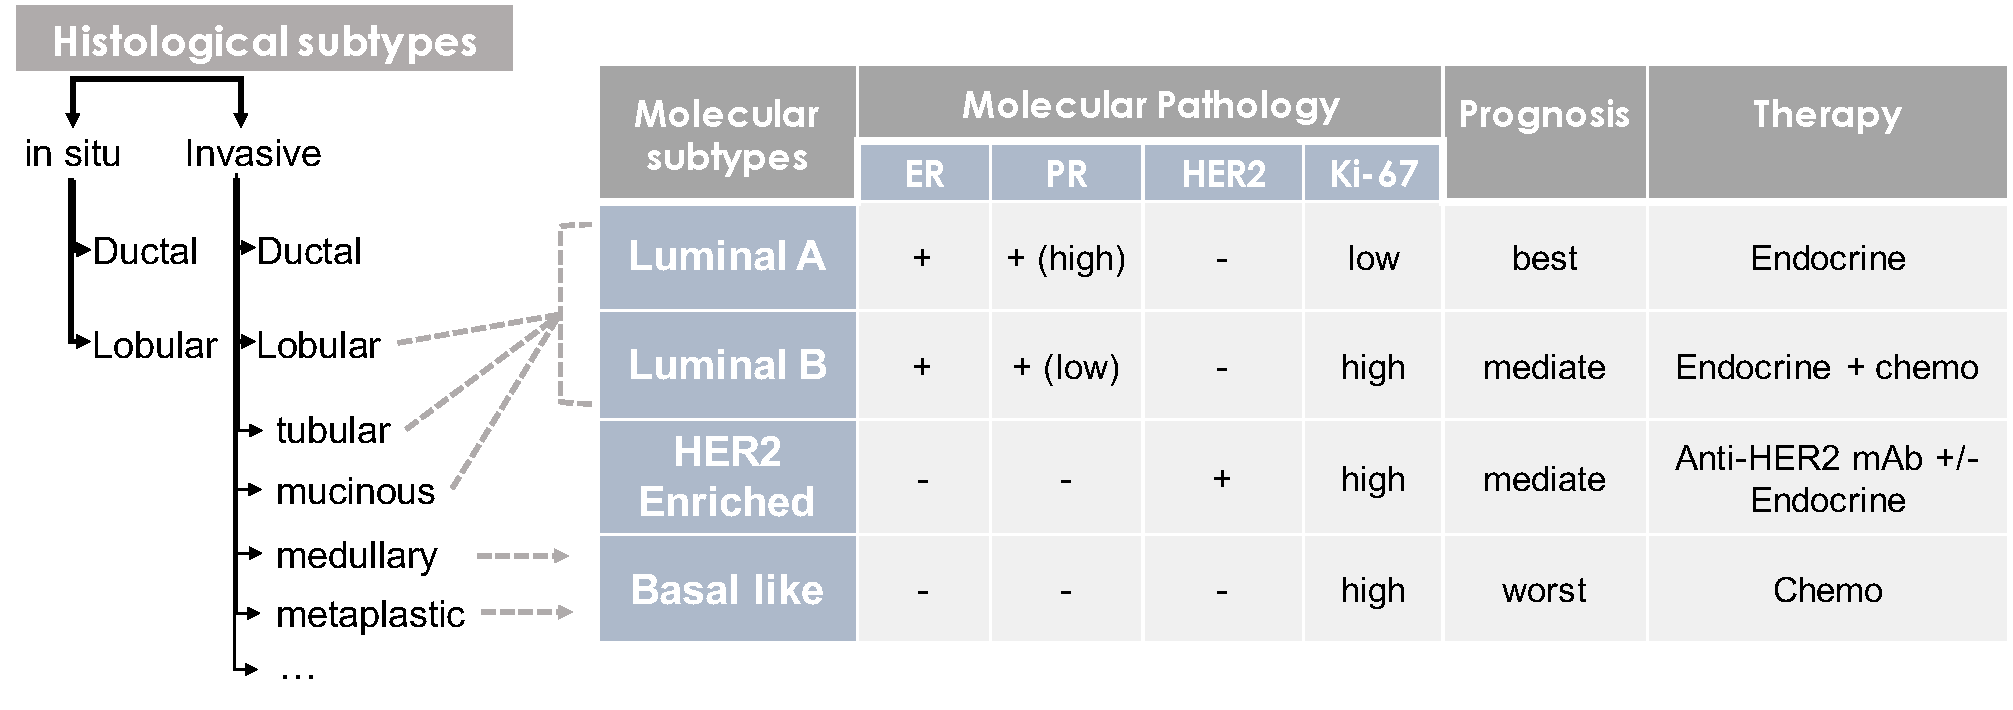
\includegraphics[width=1\linewidth]{intro.subtypes.pdf}
    \caption{Subtypes and therapeutics of breast cancer}
    \caption*{The three major subtyping systems of breast cancer, their relations with prognosis or therapy. ER: estrogen receptor, PR: progesterone receptor, HER2: human epidermal growth factor receptor 2.}
    \label{fig:example}
  \end{figure}

\section{Discussion}

In this research \citep{acar2020exploiting}

Molecular pathology is the expression of a few essential genes which determine disease behavior - e.g., in BC, being hormone receptors (ER, PR, HER2); and Ki67 as proliferation indicator, the expression of which are easily assessed by IHC or IF (immunofluorescence). Positivity is defined differently for each marker - e.g., >=1\% of stained tumor cells for ER or PR while >10\% positive cells for HER2 \citep{fragomeni2018molecular}. ER is a transcription factor (TF) canonically activated by estrogen and is one most essential indicator of endocrine therapy benefits. PR is also a steroid hormone receptor and TF, which can be induced by estrogen and in turn influence ER. Positivity in both ER and PR indicates good prognosis and endocrine responsiveness pathways \citep{lange2008challenges}. HER2 is a receptor tyrosine kinase (RTK) encoded by ERBB2 gene, which when activated, promotes survival, proliferation and invasiveness through activating the PI3K-Akt and Sos-Ras-MAPK pathways \citep{hudis2007trastuzumab}. ERBB2 amplification is detected in 15-30\% of breast cancers, and typically indicates high invasiveness. Anti-HER2 treatment is often suggested - trastuzumab, pertuzumab as monoclonal antibodies (mAb), and small molecules (gefitinib, lapatinib) targeting tyrosine kinase. Ki67 is expressed in active cell cycle, which generally reflects active proliferation and predicts poor outcomes. Chemotherapy is often suggested for tumors with high Ki67 level.

\section*{参考文献}
{\renewcommand{\bibsection}{}
\putbib
}


% 附录
% 本科生需要将附录放到声明之后,个人简历之前
\appendix
% % !TeX root = ../thuthesis-example.tex

\begin{survey}
\label{cha:survey}

\title{Title of the Survey}
\maketitle


\tableofcontents


本科生的外文资料调研阅读报告。


\section{Figures and Tables}

\subsection{Figures}

An example figure in appendix (Figure~\ref{fig:appendix-survey-figure}).

\begin{figure}
  \centering
  
\includegraphics[width=0.6\linewidth]{example-image-a.pdf}
  \caption{Example figure in appendix}
  \label{fig:appendix-survey-figure}
\end{figure}


\subsection{Tables}

An example table in appendix (Table~\ref{tab:appendix-survey-table}).

\begin{table}
  \centering
  \caption{Example table in appendix}
  \begin{tabular}{ll}
    \toprule
    File name       & Description                                         \\
    \midrule
    thuthesis.dtx   & The source file including documentaion and comments \\
    thuthesis.cls   & The template file                                   \\
    thuthesis-*.bst & BibTeX styles                                       \\
    thuthesis-*.bbx & BibLaTeX styles for bibliographies                  \\
    thuthesis-*.cbx & BibLaTeX styles for citations                       \\
    \bottomrule
  \end{tabular}
  \label{tab:appendix-survey-table}
\end{table}


\section{Equations}

An example equation in appendix (Equation~\eqref{eq:appendix-survey-equation}).
\begin{equation}
  \frac{1}{2 \uppi \symup{i}} \int_\gamma f = \sum_{k=1}^m n(\gamma; a_k) \mathscr{R}(f; a_k)
  \label{eq:appendix-survey-equation}
\end{equation}


\section{Citations}

% Example\cite{dupont1974bone} citations\cite{merkt1995rotational} in appendix
% \cite{dupont1974bone,merkt1995rotational}.


% 默认使用正文的参考文献样式;
% 如果使用 BibTeX,可以切换为其他兼容 natbib 的 BibTeX 样式。
\bibliographystyle{unsrtnat}
% \bibliographystyle{IEEEtranN}

% 默认使用正文的参考文献 .bib 数据库;
% 如果使用 BibTeX,可以改为指定数据库,如 \bibliography{ref/refs}。
\printbibliography

\end{survey}
       % 本科生:外文资料的调研阅读报告
% % !TeX root = ../thuthesis-example.tex

\begin{translation}
\label{cha:translation}

\title{书面翻译题目}
\maketitle

\tableofcontents


本科生的外文资料书面翻译。


\section{图表示例}

\subsection{图}

附录中的图片示例(图~\ref{fig:appendix-translation-figure})。

\begin{figure}
  \centering
  
\includegraphics[width=0.6\linewidth]{example-image-a.pdf}
  \caption{附录中的图片示例}
  \label{fig:appendix-translation-figure}
\end{figure}


\subsection{表格}

附录中的表格示例(表~\ref{tab:appendix-translation-table})。

\begin{table}
  \centering
  \caption{附录中的表格示例}
  \begin{tabular}{ll}
    \toprule
    文件名          & 描述                         \\
    \midrule
    thuthesis.dtx   & 模板的源文件,包括文档和注释 \\
    thuthesis.cls   & 模板文件                     \\
    thuthesis-*.bst & BibTeX 参考文献表样式文件    \\
    thuthesis-*.bbx & BibLaTeX 参考文献表样式文件  \\
    thuthesis-*.cbx & BibLaTeX 引用样式文件        \\
    \bottomrule
  \end{tabular}
  \label{tab:appendix-translation-table}
\end{table}


\section{数学公式}

附录中的数学公式示例(公式\eqref{eq:appendix-translation-equation})。
\begin{equation}
  \frac{1}{2 \uppi \symup{i}} \int_\gamma f = \sum_{k=1}^m n(\gamma; a_k) \mathscr{R}(f; a_k)
  \label{eq:appendix-translation-equation}
\end{equation}


\section{文献引用}

% 附录\cite{dupont1974bone}中的参考文献引用\cite{merkt1995rotational}示例
% \cite{dupont1974bone,merkt1995rotational}。


\appendix

\section{附录}

附录的内容。


% 书面翻译的参考文献
% 默认使用正文的参考文献样式;
% 如果使用 BibTeX,可以切换为其他兼容 natbib 的 BibTeX 样式。
\bibliographystyle{unsrtnat}
% \bibliographystyle{IEEEtranN}

% 默认使用正文的参考文献 .bib 数据库;
% 如果使用 BibTeX,可以改为指定数据库,如 \bibliography{ref/refs}。
\printbibliography

% 书面翻译对应的原文索引
% \begin{translation-index}
%   \nocite{mellinger1996laser}
%   \nocite{bixon1996dynamics}
%   \nocite{carlson1981two}
%   \bibliographystyle{unsrtnat}
%   \printbibliography
% \end{translation-index}

\end{translation}
  % 本科生:外文资料的书面翻译
% % !TeX root = ../thuthesis-example.tex

\chapter{补充内容}

附录是与论文内容密切相关、但编入正文又影响整篇论文编排的条理和逻辑性的资料,例如某些重要的数据表格、计算程序、统计表等,是论文主体的补充内容,可根据需要设置。

附录中的图、表、数学表达式、参考文献等另行编序号,与正文分开,一律用阿拉伯数字编码,
但在数码前冠以附录的序号,例如“图~\ref{fig:appendix-figure}”,
“表~\ref{tab:appendix-table}”,“式\eqref{eq:appendix-equation}”等。


\section{插图}

% 附录中的插图示例(图~\ref{fig:appendix-figure})。

\begin{figure}
  \centering
  
\includegraphics[width=0.6\linewidth]{example-image-a.pdf}
  \caption{附录中的图片示例}
  \label{fig:appendix-figure}
\end{figure}


\section{表格}

% 附录中的表格示例(表~\ref{tab:appendix-table})。

\begin{table}
  \centering
  \caption{附录中的表格示例}
  \begin{tabular}{ll}
    \toprule
    文件名          & 描述                         \\
    \midrule
    thuthesis.dtx   & 模板的源文件,包括文档和注释 \\
    thuthesis.cls   & 模板文件                     \\
    thuthesis-*.bst & BibTeX 参考文献表样式文件    \\
    thuthesis-*.bbx & BibLaTeX 参考文献表样式文件  \\
    thuthesis-*.cbx & BibLaTeX 引用样式文件        \\
    \bottomrule
  \end{tabular}
  \label{tab:appendix-table}
\end{table}


\section{数学表达式}

% 附录中的数学表达式示例(式\eqref{eq:appendix-equation})。
\begin{equation}
  \frac{1}{2 \uppi \symup{i}} \int_\gamma f = \sum_{k=1}^m n(\gamma; a_k) \mathscr{R}(f; a_k)
  \label{eq:appendix-equation}
\end{equation}


\section{文献引用}

% 附录\cite{dupont1974bone}中的参考文献引用\cite{zhengkaiqing1987}示例
% \cite{dupont1974bone,zhengkaiqing1987}。

\printbibliography


% 致谢
% !TeX root = ../thuthesis-example.tex
\renewcommand{\chaptermark}[1]{\markboth{#1}{}} 
\begin{acknowledgements}
  \markboth{致谢}{}
  衷心感谢导师×××教授和物理系××副教授对本人的精心指导。他们的言传身教将使我终生受益。

  在美国麻省理工学院化学系进行九个月的合作研究期间,承蒙 Robert Field 教授热心指导与帮助,不胜感激。

  感谢×××××实验室主任×××教授,以及实验室全体老师和同窗们学的热情帮助和支持!

  本课题承蒙国家自然科学基金资助,特此致谢。
  test test
\end{acknowledgements}


% 声明
\statement
% 将签字扫描后的声明文件 scan-statement.pdf 替换原始页面
% \statement[file=scan-statement.pdf]
% 本科生编译生成的声明页默认不加页脚,插入扫描版时再补上;
% 研究生编译生成时有页眉页脚,插入扫描版时不再重复。
% 也可以手动控制是否加页眉页脚
% \statement[page-style=empty]
% \statement[file=scan-statement.pdf, page-style=plain]
% 个人简历、在学期间完成的相关学术成果
% 本科生可以附个人简历,也可以不附个人简历
% !TeX root = ../thuthesis-example.tex

\begin{resume}

  \section*{个人简历}

  197× 年 ×× 月 ×× 日出生于四川××县。

  1992 年 9 月考入××大学化学系××化学专业,1996 年 7 月本科毕业并获得理学学士学位。

  1996 年 9 月免试进入清华大学化学系攻读××化学博士至今。


  \section*{在学期间完成的相关学术成果}

  \subsection*{1  学术论文}

  \begin{achievements}
    \item Yang Y, Ren T L, Zhang L T, et al. Miniature microphone with silicon-based ferroelectric thin films[J]. Integrated Ferroelectrics, 2003, 52:229-235.
    \item 杨轶, 张宁欣, 任天令, 等. 硅基铁电微声学器件中薄膜残余应力的研究[J]. 中国机械工程, 2005, 16(14):1289-1291.
    \item 杨轶, 张宁欣, 任天令, 等. 集成铁电器件中的关键工艺研究[J]. 仪器仪表学报, 2003, 24(S4):192-193.
    \item Yang Y, Ren T L, Zhu Y P, et al. PMUTs for handwriting recognition. In press[J]. (已被Integrated Ferroelectrics录用)
  \end{achievements}


  \subsection*{2  专利}

  \begin{achievements}
    \item 任天令, 杨轶, 朱一平, 等. 硅基铁电微声学传感器畴极化区域控制和电极连接的方法: 中国, CN1602118A[P]. 2005-03-30.
    \item Ren T L, Yang Y, Zhu Y P, et al. Piezoelectric micro acoustic sensor based on ferroelectric materials: USA, No.11/215, 102[P]. (美国发明专利申请号.)
  \end{achievements}

  \subsection*{3  奖项}

  \begin{achievements}
    \item 任天令, 杨轶, 朱一平, 等. 硅基铁电微声学传感器畴极化区域控制和电极连接的方法: 中国, CN1602118A[P]. 2005-03-30.
    \item Ren T L, Yang Y, Zhu Y P, et al. Piezoelectric micro acoustic sensor based on ferroelectric materials: USA, No.11/215, 102[P]. (美国发明专利申请号.)
  \end{achievements}

\end{resume}


% 指导教师/指导小组评语
% 本科生不需要
% !TeX root = ../thuthesis-example.tex

\begin{commentsbasic}
% \begin{comments}[name = {指导小组评语}]
% \begin{comments}[name = {Comments from Thesis Supervisor}]
% \begin{comments}[name = {Comments from Thesis Supervision Committee}]

  论文提出了……

\end{commentsbasic}

% !TeX root = ../thuthesis-example.tex

\begin{commentsclinic}
% \begin{comments}[name = {指导小组评语}]
% \begin{comments}[name = {Comments from Thesis Supervisor}]
% \begin{comments}[name = {Comments from Thesis Supervision Committee}]

  论文提出了……

\end{commentsclinic}

% 答辩委员会决议书
% 本科生不需要
% !TeX root = ../thuthesis-example.tex

\begin{resolution}

  论文提出了……

  论文取得的主要创新性成果包括:

  1. ……

  2. ……

  3. ……

  论文工作表明作者在×××××具有×××××知识,具有××××能力,论文××××,答辩××××。

  答辩委员会表决,(×票/一致)同意通过论文答辩,并建议授予×××(姓名)×××(门类)学博士/硕士学位。

\end{resolution}

% !TeX root = ../thuthesis-example.tex

\begin{loa}

  letter of authorization
  I, Xinghua Lu, hereby certify that the contents of research work described in the attached thesis were accomplished by Tsinghua scholar Qiao Jin, and I authorize the scholar to use the contents of this research work in his thesis to partially fulfill the requirements of a Doctor of Medicine (M.D.) degree at Tsinghua University School of Medicine.

\end{loa}

% 本科生的综合论文训练记录表(扫描版)
% \record{file=scan-record.pdf}

\end{document}
